\begin{exercise}
      {ID-4a7c8962946e2dc887d2dc9cdf3d6c388927b2fb}
      {Pfeilspitze}
  \ifproblem\problem\par
    Berechne den Flächeninhalt der abgebildeten Figur.\par
    \begin{center}
      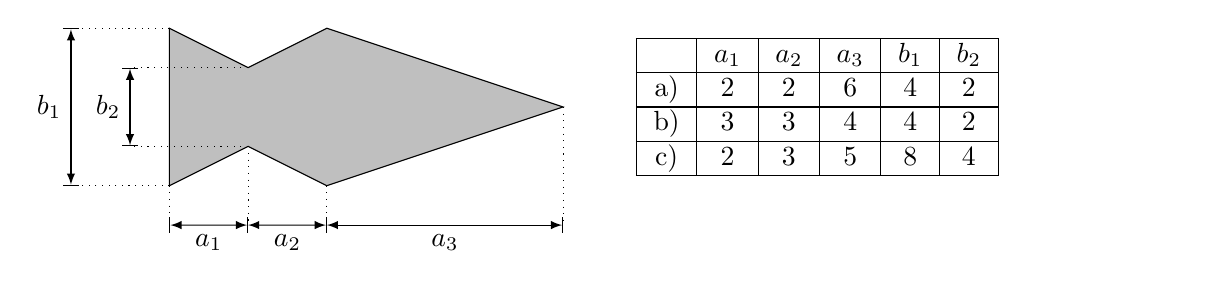
\begin{tikzpicture}[scale=0.5]
        \filldraw[fill=black!25!white, draw=black]
          (0, 0)   coordinate (A)
          -- (2, 1)   coordinate (B)
          -- (4, 0)   coordinate (C)
          -- (10, 2)  coordinate (D)
          -- (4, 4)   coordinate (E)
          -- (2, 3)   coordinate (F)
          -- (0, 4)   coordinate (G)
          -- cycle;
        % Beschriftung (unten)
        \draw[style=dotted] (A) -- ++(270:1) coordinate (H1);
        \draw[style=dotted] (B) -- ++(270:2) coordinate (H2);
        \draw[style=dotted] (C) -- ++(270:1) coordinate (H3);
        \draw[style=dotted] (D) -- ++(270:3) coordinate (H4);
        \draw[|<->|, >=latex] (H1) -- node[below]{$a_1$} (H2);
        \draw[<->|,  >=latex] (H2) -- node[below]{$a_2$} (H3);
        \draw[<->|,  >=latex] (H3) -- node[below]{$a_3$} (H4);
        % Beschriftung (links)
        \draw[style=dotted] (F) -- ++(180:3) coordinate (H1);
        \draw[style=dotted] (B) -- ++(180:3) coordinate (H2);
        \draw[style=dotted] (G) -- ++(180:2.5) coordinate (H3);
        \draw[style=dotted] (A) -- ++(180:2.5) coordinate (H4);
        \draw[|<->|, >=latex] (H1) -- node[left]{$b_2$} (H2);
        \draw[|<->|, >=latex] (H3) -- node[left]{$b_1$} (H4);
        % Tabelle
        \node[right=8mm] at (D)
        {%
          \begin{minipage}{6.8cm}
            \begin{tabular}{|c|c|c|c|c|c|}
              \hline
                 & $a_1$ & $a_2$ & $a_3$ & $b_1$ & $b_2$ \\
              \hline
              a) & \sicm{2} & \sicm{2} & \sicm{6} & \sicm{4} & \sicm{2} \\
              \hline
              b) & \sicm{3} & \sicm{3} & \sicm{4} & \sicm{4} & \sicm{2} \\
              \hline
              c) & \sicm{2} & \sicm{3} & \sicm{5} & \sicm{8} & \sicm{4} \\
              \hline
            \end{tabular}%
          \end{minipage}%
        };
      \end{tikzpicture}%
    \end{center}
  \fi
  %\ifoutline\outline\par
  %  \begingroup
  %    \dimen1=5cm%
  %    \begin{minipage}{\dimen1}%
  %      \begin{tikzpicture}%
  %      \end{tikzpicture}%
  %    \end{minipage}%
  %    \dimen2=\linewidth%
  %    \advance\dimen2 by -\dimen1%
  %    \begin{minipage}{\dimen2}%
  %      \setlength{\abovedisplayskip}{0pt}%
  %      \begin{equation*}
  %      \end{equation*}
  %    \end{minipage}%
  %  \endgroup
  %\fi
  \ifoutcome\outcome\par
    \begin{equation*}
      \text{a)~}A=\sicmm{24}
      \qquad
      \text{b)~}A=\sicmm{26}
      \qquad
      \text{c)~}A=\sicmm{50}
    \end{equation*}
  \fi
\end{exercise}
